\section{Methods}

We seek to extend the method of \cite{zhao2011large} to deep convolutional
neural networks.  We show that by using soft labels, our model can achieve
better classification performance.

% In addition, we also see if soft labels can
% help reduce the required number of training examples.

%Based on the work of
%\cite{hinton2015distilling}, we will see if we can reduce the architectural
%complexity of our network (thus reducing training and evaluation time).

We compare different schemes for obtaining soft labels for ImageNet
categories.  In doing so, we explore semantic similarity measures derived from
word embeddings trained on large amounts of text, knowledge bases such as 
WordNet, as well as visual similarity metrics and compare them against each
other.


\subsection{Soft Labels}
\label{sec:soft_labels}

\begin{table}[!tb]
  \centering
  \begin{tabular}{|c|c|c|c|c|}
    \hline
      & Donkey & Mule & Truck & Cat \\
    \hline
      ``Donkey'' 1-hot & 1 & 0 & 0 & 0 \\
    \hline
      ``Donkey'' soft & 0.8 & 0.15 & 0.0 & 0.05 \\
    \hline
  \end{tabular}
  \caption{
    A toy example of a 1-hot label compared to a soft label.
  }
  \label{tbl:soft_labels}
\end{table}

Traditionally when training a classifier, the loss function would be computed
by comparing the prediction values against a 1-hot label vector.
A 1-hot label means that the correct (ground truth) category is given a value
of 1 and all other categories are given a value of 0.
When the classifier makes an error, it is not given any ``partial credit''
based on the semantic relevance of its mistake.

On the contrary, soft labels provide a real-valued distribution over
the object categories. Thus, the classifier is not penalized as
heavily for making a semantically relevant error (e.g. misclassifying
a ``donkey'' as a ``mule'') as it would be for a completely incorrect
prediction (e.g. misclassifying a ``truck'' as a ``cat''). The use of
soft labels also encourages assigning a small amount of probability
mass to semantically-related classes. A model which is able to assign
probability mass to semantically-related classes consequently has a richer
understanding of the image than a model which assigns high probability mass to
unrelated classes. An example is shown in Table \ref{tbl:soft_labels}.

A soft labeling scheme can be visualized by an \emph{affinity matrix}. Figure
\ref{fig:aff-5_1} shows a five class affinity matrix. For affinity matrix $A$,
element $A_{ij}$ is the similarity (i.e. \emph{affinity}) between class $i$ and
class $j$. Affinity matrices are typically symmetric (i.e. $A_{ij} = A_{ji}$ for
all $i, j$), although we violate this constraint word2vec similarity scheme (for
an example see Section \ref{word2vec}).

\begin{figure}[!tb]
%\begin{figure}[t]
  \centering
  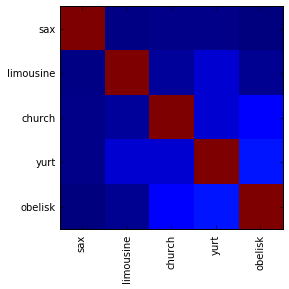
\includegraphics[width=0.4\textwidth]{figs/aff-5_1.png}
  \caption{
      Affinity matrix for five ImageNet classes computed from word2vec word
      similarity. Note that \emph{church}, \emph{yurt}, and
      \emph{obelisk} have high similarity, due to their building nature, while
      \emph{limousine} and \emph{sax} have low similarity to most other classes.
  }
  \label{fig:aff-5_1}
\end{figure}

\subsection{Linguistic Semantic Similarity}


\subsubsection{WordNet}

WordNet is a large database of English words grouped into synonym sets called
sysnets \cite{miller1995wordnet}.
The sysnets are related hierarchically with semantic and conceptual links, such
as hypernyms (``is a'') and meronyms (``part of'') relationships.

Using the distance metric in equation \ref{eq:wordnet_dist}, we follow the work
of \cite{fergus2010semantic} and \cite{zhao2011large} for defining soft labels
for a deep CNN classifier. We experimentally test a wide variety of
hyperparameters and values for $\kappa$, which measures how diffuse or sparse
the similarity distribution is.  Moreover, we further analyze the performance
tradeoffs between hyperonym and meronym relations.  Using both relationships has
been introduced in \cite{marszalek2007semantic} for hierarchical classification,
but to the best of our knowledge has not been used in comparing soft label
performance before \textbf{(DO WE DO THIS???)}.


\subsubsection{Word Embeddings} \label{word2vec}

A word embedding maps each word in a lexicon to a continuous
real-valued vector. This nature of this mapping is often guided by the
distributional hypothesis introduced in
\cite{harris1954distributional}, which states that a word can be
understood by the context it appears in. Assuming this hypothesis, a
desirable mapping is one that maps words which appear in similar
contexts to nearby locations in the vector space.

Popular methods for computing word embeddings such as word2vec
\cite{mikolov2013distributed} and GloVe \cite{pennington2014glove} have been
shown to capture such properties.  However, \cite{levy2014dependency} shows that
when context is varied, the notion of similarity between words also changes. For
example, when context is taken to be neighboring words, words close in the
vector space tend to be \emph{topically} similar. Conversely, when context is
defined via \emph{linguistic dependencies}, nearby words tend to be
\emph{semantically} similar. We examine the effect word context has on semantic
label sharing for image classification.

To compute the similarity between two labels with word vectors, we compute the
cosine similarity between the two vectors. We take the additional following step
to normalize the similarity scores of the off-diagonal. For a label $i$, we
normalize all of the off-diagonal similarity scores to sum to $k$, where $k$ is
a hyperparameter. We found the value of $k = 0.5$ to work the best. Typically
when normalizing a distribution, $k$ is taken to be 1. However, when the
similarity distribution is very sparse, this can mean that the similarity
between two classes can be close to a 1.0, which confuses learning. In order to
guard against this, we enfornce the contraint that the similarity between two
distinct classes cannot be greater than $k$.

The result of this process is that the affinity matrix is no longer symmetric.
The largest asymmetries occur when one class is not similar to any other classes
(e.g. \emph{sax}), and assigns uniform probability mass to all other classes.
Meanwhile, another class (e.g. \emph{yurt}), who has high similarity to other
classes, assigns near-zero probability mass to \emph{sax}.

\subsection{Visual Similarity}

A main focus of our work is to exploit information embedded in natural language
to aid in visual classification.  However, it has been shown that lingustic
semantics do not always work well in modeling visual similarity
\cite{li2010building}. As an example given in \cite{li2010building}, WordNet
does not capture the correlation between ``tower'' and ``business district''.
To this end, we explore soft labeling schemes based on visual similarity
and compare the performance and label distributions to those of the lingustic
schemes.

% By better understanding the relationship between linguistic similarity
% and the visual representations learned by a CNN, we hope to explore improved
% ways of defining and weighting soft labels.  We use several existing
% methods to compute the similarities between different image categories.

First, we will take the average GIST descriptor \cite{oliva2001modeling} values
for each category across all images in the training data set. We will use the
scaled similarity between these descriptors as a distribution across the soft
labels.
Since GIST is a global descriptor, we expect it to capture more of the
background contextual information rather than similarities between the objects
themselves.

To better represent the categories directly, we can also experiment with
visual word clusters mined from images of different object categories.
We expect that clustering SIFT descriptors \cite{lowe1999object} should work
reasonably well.
The similarity metric can be defined as the distance between the cluster
centroids into which the images of different categories fall.
We can also explore using visual vocabulary trees, introduced by
\cite{nister2006scalable}.

We can investigate many other methods. The most notable and relevant to our
work is \cite{li2010building}, who have successfully used their visual
similarity approach for improving hierarchical image classification.
We can also explore other works in unsupervised clustering, including most
recent advancements using deep neural networks in unsupervised visual
clustering
(Jianwei Yang, Devi Parikh, and Dhruv Batra, 2016 - not yet published).

% Possibly the trained experts thing?
